\documentclass[11pt]{article} 
%\usepackage{amsbsy} % for \boldsymbol and \pmb 
%\usepackage{graphicx} % To include pdf files!
\usepackage{amsmath}
\usepackage{amsbsy}
\usepackage{amsfonts}
\usepackage{enumerate}
\usepackage[colorlinks=true, pdfstartview=FitV, linkcolor=blue, citecolor=blue, urlcolor=blue]{hyperref} % For links
\usepackage{fullpage}
\pagestyle{empty}
\usepackage{pgf,pgfplots,tikz}
\usepackage{amsmath,amssymb,amsthm}
\usepackage{tikz}
\newcommand{\overrightharp}[1]{\hat{#1}}
\DeclareMathOperator{\proj}{proj}
\DeclareMathOperator{\years}{years}
\DeclareMathOperator{\cm}{cm}
\newcommand{\vct}{\mathbf}
\newcommand{\vctproj}[2][]{\proj_{{#1}}\vct{#2}}
\newtheorem{theorem}{Theorem}
\DeclareMathOperator{\m}{m}
\DeclareMathOperator{\kg}{kg}
\DeclareMathOperator{\N}{N}
\DeclareMathOperator{\Or}{or}
\DeclareMathOperator{\J}{J}
\DeclareMathOperator{\s}{s}
\DeclareMathOperator{\g}{g}
\DeclareMathOperator{\W}{W}
\DeclareMathOperator{\Heatoms}{He\hspace{1mm} atoms}
\DeclareMathOperator{\MeV}{MeV}
\DeclareMathOperator{\tr}{tr}
\newcommand{\norm}[1]{\left\lVert#1\right\rVert}
\usepackage{graphicx}
\newcommand{\abs}[1]{\lvert#1\rvert}
\DeclareMathOperator{\diverge}{div\,}
\DeclareMathOperator{\curl}{curl\,}
\title{\textbf{JCP321 POTW4}
\author{Maxim Piatine\\1005303100}}
\date{}
\DeclareMathOperator{\lineint}{\int \mathbf{v}\cdot d\mathbf{l}}
\DeclareMathOperator{\surfint}{\int \mathbf{v}\cdot d\mathbf{a}}
\begin{document}
\maketitle
\section*{(a)}
The question is asking to define a wave function $\Psi(x,0)$ where the particles are equally likely to be found anywhere in $x\in[\frac{a}{4},\frac{3a}{4}]$. $\Psi(x,0)$ needs to be strictly real, positive function. Thus, the function I went with is 
\[\Psi(x,0)=
\begin{cases}
    A(x-\frac{a}{4})(\frac{3a}{4}-x) & , \text{if } x\in[\frac{a}{4},\frac{3a}{4}]\\
    0 & , \text{otherwise}
\end{cases}\]
\begin{center}
    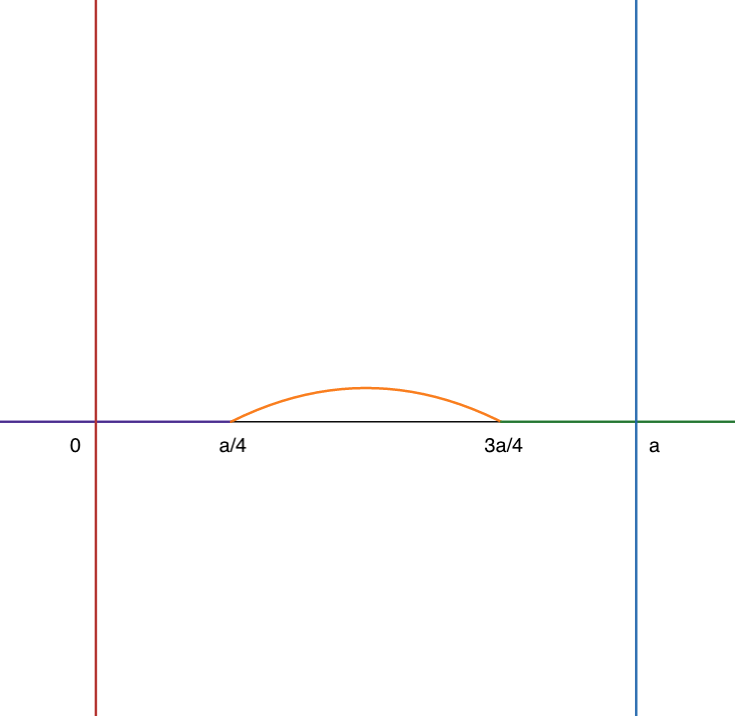
\includegraphics[width=7cm]{abc.png}
\end{center}
The wave function is continuous, differentiable, and positive. 
\[\int^{\infty}_{-\infty}|\Psi(x,0)|^2dx = 1\]
\[=\int_{-\infty}^{\frac{a}{4}}0 dx+\int^{\frac{3a}{4}}_{\frac{a}{4}}  A^2(x-\frac{a}{4})^2(\frac{3a}{4}-x)^2 dx+\int_{\frac{3a}{4}}^{\infty}0dx=\int^{\frac{3a}{4}}_{\frac{a}{4}} A^2(x-\frac{a}{4})^2(\frac{3a}{4}-x)^2 dx=A^2\int^{\frac{3a}{4}}_{\frac{a}{4}} (x-\frac{a}{4})^2(\frac{3a}{4}-x)^2 dx\]
After all the expansions and computations we are left with this integral:
\[=A^2\int^{\frac{3a}{4}}_{\frac{a}{4}} x^4-2ax^3+\frac{11a^2x^2}{8}-\frac{3a^3x}{8}+\frac{9a^4}{256} dx=A^2\left[ 
\frac{x^5}{5}-\frac{ax^4}{2}+\frac{11a^2x^2}{24}-\frac{3a^3x^2}{16}+\frac{9a^4x}{256}
\right]^{\frac{3a}{4}}_{\frac{a}{4}}\]
\[=A^2\left[\frac{243a^5}{5120}-\frac{81a^5}{512}+...+\frac{3a^5}{256}-\frac{9a^5}{1024}\right]=A^2[\frac{a^5}{960}]=1\]
\[\Rightarrow A^2=\frac{960}{a^5} \Rightarrow A=\frac{8\sqrt{15}}{a^\frac{5}{2}}\]
\[\Psi(x,0)=\begin{cases}
    \frac{8\sqrt{15}}{\sqrt{a^5}}(x-\frac{a}{4})(\frac{3a}{4}-x) & ,\text{if } x\in[\frac{a}{4},\frac{3a}{4}]\\
    0 & ,\text{otherwise}
\end{cases}\]

\section*{(b)}
\[c_n=\sqrt{\frac{2}{a}}\int_{\frac{a}{4}}^{\frac{3a}{4}}\sin{(\frac{n\pi x}{a})}\Psi(x,0) dx=
\sqrt{\frac{2}{a}}\int_{\frac{a}{4}}^{\frac{3a}{4}}\sin{(\frac{n\pi x}{a})}\left(\frac{8\sqrt{15}}{\sqrt{a^5}}(x-\frac{a}{4})(\frac{3a}{4}-x) \right)dx\] 

\[=\sqrt{\frac{1920}{a^6}}\int_{\frac{a}{4}}^{\frac{3a}{4}}
\sin{(\frac{n\pi x}{a})}(x-\frac{a}{4})(\frac{3a}{4}-x)dx=
\frac{1}{a^3}\sqrt{1920}\int_{\frac{a}{4}}^{\frac{3a}{4}}
\sin{(\frac{n\pi x}{a})}(x-\frac{a}{4})(\frac{3a}{4}-x)dx\]
Using integration by parts, substituting, computing, and simplifying; we get to this:
\[=\frac{1}{a^3}\sqrt{1920}
\left[
\frac{-a^3n\pi \sin{(\frac{3n\pi}{4})}-a^3n\pi \sin{(\frac{n\pi}{4})}-4a^3\cos{(\frac{3n\pi}{4})}+4a^3\cos{(\frac{n\pi}{4})}}
{2n^3\pi^3}
\right]\]

\[c_n=-\frac{\sqrt{1920}}{2n^3\pi^3}
\left[ 
n\pi\sin{(\frac{3n\pi}{4})} + n\pi \sin{(\frac{n\pi}{4})}+ 
4\cos{(\frac{3n\pi}{4})}-4\cos{(\frac{n\pi}{4})}
\right]\]

Therefore, the general solution to the time-dependent Schrodinger equation is a linear combination of stationary states:
\[\Psi(x,t)=\sum_{n=1}^{\infty}c_n \sqrt{\frac{2}{a}}\sin{(\frac{n\pi x}{a})}\exp{\left(-i(\frac{n^2\pi^2\hbar}{2ma^2})t\right)}\]

\[\Psi(x,t)=-\sqrt{\frac{{960}}{a}}\frac{1}{\pi^3}
\sum^{\infty}_{n=1}
\frac{1}{n^3}\left[ 
n\pi\sin{(\frac{3n\pi}{4})} + n\pi \sin{(\frac{n\pi}{4})}+ 
4\cos{(\frac{3n\pi}{4})}-4\cos{(\frac{n\pi}{4})}
\right]
\sin{(\frac{n\pi x}{a})}\exp{\left(-i(\frac{n^2\pi^2\hbar}{2ma^2})t\right)}\]
Time independent:
\[\Psi(x,0)=-\sqrt{\frac{{960}}{a}}\frac{1}{\pi^3}
\sum^{\infty}_{n=1}
\frac{1}{n^3}\left[ 
n\pi\sin{(\frac{3n\pi}{4})} + n\pi \sin{(\frac{n\pi}{4})}+ 
4\cos{(\frac{3n\pi}{4})}-4\cos{(\frac{n\pi}{4})}
\right]
\sin{(\frac{n\pi x}{a})}\]

\section*{(c)}
Using the $c_n$ that we've found:
\[c_n=-\frac{\sqrt{1920}}{2n^3\pi^3}
\left[ 
n\pi\sin{(\frac{3n\pi}{4})} + n\pi \sin{(\frac{n\pi}{4})}+ 
4\cos{(\frac{3n\pi}{4})}-4\cos{(\frac{n\pi}{4})}
\right]\]
We find $c_1$; meaning $n=1$:
\[c_1=-\frac{\sqrt{1920}}{2(1)^3\pi^3}
\left[ 
(1)\pi \left(\sin{(\frac{3(1)\pi}{4})} + \sin{(\frac{(1)\pi}{4})}\right)+ 
4\left(\cos{(\frac{3(1)\pi}{4})}-\cos{(\frac{(1)\pi}{4})}\right)
\right]\]

\[=-\frac{\sqrt{1920}}{2\pi^3}\left[\pi(\frac{\sqrt{2}}{2}+\frac{\sqrt{2}}{2})+4(-\frac{\sqrt{2}}{2}-\frac{\sqrt{2}}{2})\right]=-\frac{\sqrt{1920}}{2\pi^3}\left[ \sqrt{2}\pi -4\sqrt{2}\right]=0.857787\]

We find $c_2$; at $n=2$:
\[c_2=-\frac{\sqrt{1920}}{2(2)^3\pi^3}
\left[ 
(2)\pi \left(\sin{(\frac{3(2)\pi}{4})} + \sin{(\frac{(2)\pi}{4})}\right)+ 
4\left(\cos{(\frac{3(2)\pi}{4})}-\cos{(\frac{(2)\pi}{4})}\right)
\right]\]

\[=-\frac{\sqrt{1920}}{16\pi^3}
\left[ 
2\pi \left(\sin{(\frac{3\pi}{2})} + \sin{(\frac{\pi}{2})}\right)+ 
4\left(\cos{(\frac{3\pi}{2})}-\cos{(\frac{\pi}{2})}\right)
\right]=-\frac{\sqrt{1920}}{16\pi^3}\left[ 2\pi(-1+1)+4(0-0)\right]=0\]

\end{document}
